%==============================================================
%  EE201 -- Circuit Theory I
%  Lecture 7 : Circuit Graphs and the Incidence Matrix -- slides
%  M. Mert Ankaralı, METU EEE
%
%  Compile:  ./build.sh      (or: pdflatex EE201_Lecture_7_slides.tex, twice)
%  Same colour code as the handout:
%      charge = purple, current = blue, voltage = orange, power = green
%==============================================================
\documentclass[11pt,aspectratio=169]{beamer}

\usepackage[T1]{fontenc}
\usepackage[utf8]{inputenc}
\usepackage[english]{babel}
\usepackage{lmodern}
\usepackage{amsmath,amssymb}
\usepackage{booktabs}
\usepackage{array}
\usepackage{colortbl}
\usepackage{tikz}
\usepackage[american,siunitx]{circuitikz}
\usetikzlibrary{matrix,arrows.meta,positioning,calc,decorations.pathreplacing,decorations.pathmorphing,decorations.markings}
\usetikzlibrary{overlay-beamer-styles}

%-------------------- plain METU-flavoured theme --------------
\usetheme{default}
\usecolortheme{default}
\useinnertheme{rectangles}
\setbeamertemplate{navigation symbols}{}
\setbeamertemplate{itemize items}[square]
\setbeamerfont{frametitle}{size=\large,series=\bfseries}
\setbeamerfont{title}{size=\LARGE,series=\bfseries}

\definecolor{metured}{RGB}{155,27,48}
\definecolor{metugray}{RGB}{88,89,91}
\definecolor{metulight}{RGB}{243,240,241}
\definecolor{ccur}{RGB}{0,102,170}
\definecolor{cvolt}{RGB}{214,120,0}
\definecolor{cpow}{RGB}{23,128,74}
\definecolor{ccharge}{RGB}{124,60,160}
\definecolor{cflux}{RGB}{0,138,138}
\definecolor{copper}{RGB}{184,98,30}

\setbeamercolor{structure}{fg=metured}
\setbeamercolor{frametitle}{fg=metured,bg=}
\setbeamercolor{title}{fg=metured}
\setbeamercolor{normal text}{fg=black!88}
\setbeamercolor{block title}{fg=white,bg=metured}
\setbeamercolor{block body}{bg=metulight}
\setbeamercolor{alerted text}{fg=metured}

\setbeamertemplate{frametitle}{%
  \vspace{0.55em}%
  \usebeamerfont{frametitle}\usebeamercolor[fg]{frametitle}\insertframetitle\par
  \vspace{-0.2em}{\color{metured}\rule{\textwidth}{1pt}}\par\vspace{-0.2em}}

\setbeamertemplate{footline}{%
  \hbox{\begin{beamercolorbox}[wd=\paperwidth,ht=2.4ex,dp=1.4ex,leftskip=1.2em,rightskip=1.2em]{}%
  \tiny\color{metugray}\coursecode\ \textbar\ Lecture 7: Circuit Graphs and the Incidence Matrix
  \hfill \insertframenumber/\inserttotalframenumber
  \end{beamercolorbox}}}

%-------------------- macros ----------------------------------
\newcommand{\coursecode}{EE201}
\newcommand{\term}{Fall 2026--2027}
\newcommand{\Icol}[1]{\textcolor{ccur}{#1}}
\newcommand{\Vcol}[1]{\textcolor{cvolt}{#1}}
\newcommand{\Pcol}[1]{\textcolor{cpow}{#1}}
\newcommand{\Qcol}[1]{\textcolor{ccharge}{#1}}
\newcommand{\Fcol}[1]{\textcolor{cflux}{#1}}
\newcommand{\uni}[1]{\,\mathrm{#1}}
\newcommand{\A}{\uni{A}} \newcommand{\V}{\uni{V}}
\newcommand{\W}{\uni{W}} \newcommand{\J}{\uni{J}}
\newcommand{\Cb}{\uni{C}} \newcommand{\s}{\uni{s}}
\newcommand{\Wb}{\uni{Wb}} \newcommand{\Hy}{\uni{H}}
\newcommand{\Sie}{\uni{S}}


\ctikzset{bipoles/length=0.9cm, label/align=straight,
          bipoles/generic/height=0.28, bipoles/generic/width=0.62}
\tikzset{
  iar/.style={-{Stealth[length=2.2mm]}, ccur, thick},
  glab/.style={font=\footnotesize, text=metured},
  ttl/.style={font=\scriptsize\bfseries, text=metugray},
  capn/.style={font=\scriptsize, text=metugray, align=center},
  nlab/.style={circle, draw=metured, text=metured, font=\scriptsize, inner sep=0.7pt},
  blab/.style={font=\footnotesize, text=black!80},
  gbr/.style={black!75, thick, postaction={decorate, decoration={markings,
      mark=at position 0.56 with {\arrow{Stealth[length=2.5mm]}}}}},
  hal/.style={draw=cpow!60, line width=6pt, opacity=0.35, line cap=round, line join=round},
  halo/.style={circle, fill=metured!16, minimum size=0.95cm},
  elem/.style={draw=metugray, thick, fill=metulight},
  bigarr/.style={-{Stealth[length=3mm]}, very thick, metugray},
}

\newcommand{\nd}[1]{\tikz[baseline=(c.base)]\node[nlab](c){#1};}
\newcommand{\brarr}[4]{%
  \draw[iar] ($(#1)!0.34!(#2)!0.34cm!#3:(#2)$) -- ($(#1)!0.66!(#2)!0.34cm!#3:(#2)$);
  \node[blab] at ($(#1)!0.5!(#2)!0.66cm!#3:(#2)$) {#4};}
\newcommand{\gbranch}[4]{%
  \draw[gbr] (#1) -- (#2);
  \node[blab] at ($(#1)!0.5!(#2)!0.28cm!#3:(#2)$) {#4};}
%  An incidence matrix with node labels on the left and branch numbers on top.
%  #1 name, #2 number of columns, #3 node labels, #4 rows (entries separated by \&),
%  #5 extra TikZ code drawn on top (may refer to the cells #1-i-j)
\newcommand{\incmat}[5]{%
  \begin{tikzpicture}[baseline={([yshift=-0.6ex]#1.center)}]
    \matrix (#1) [matrix of math nodes, ampersand replacement=\&,
                  left delimiter={[}, right delimiter={]}, inner sep=1pt,
                  column sep=0.45em,
                  nodes={text width=1.35em, align=right, minimum height=1.25em,
                         inner sep=1pt}] {#4};
    \foreach \j in {1,...,#2}
      \node[font=\scriptsize, text=metugray, anchor=south east, inner sep=1pt]
        at ([yshift=2pt]#1-1-\j.north east) {\j};
    \foreach \lab [count=\i] in {#3}
      \node[nlab, left=11pt] at (#1.west |- #1-\i-1) {\lab};
    #5
  \end{tikzpicture}}
\newcommand{\bridgecoords}{%
  \coordinate (n1) at (0,1.7);  \coordinate (n2) at (-1.5,0);
  \coordinate (n3) at (1.5,0);  \coordinate (n4) at (0,-1.7);}
\newcommand{\bridgenodes}{%
  \foreach \k/\pos in {1/above, 2/left, 3/right, 4/below}
    {\fill[metured] (n\k) circle (2.2pt); \node[nlab, \pos=3pt] at (n\k) {\k};}}
\newcommand{\bridgecircuit}{%
  \draw (n1) to[generic] (n2);  \draw (n1) to[generic] (n3);
  \draw (n3) to[generic] (n2);  \draw (n2) to[generic] (n4);
  \draw (n3) to[generic] (n4);
  \coordinate (s6) at (-2.6,-1.7); \coordinate (e6) at (-2.6,1.7);
  \draw (n4) -- (s6) to[generic] (e6) -- (n1);}
\newcommand{\bridgegraph}{%
  \gbranch{n1}{n2}{-90}{1}  \gbranch{n1}{n3}{90}{2}  \gbranch{n3}{n2}{-90}{3}
  \gbranch{n2}{n4}{-90}{4}  \gbranch{n3}{n4}{90}{5}
  \draw[gbr] (n4) to[out=180, in=180, looseness=2.3] (n1);
  \node[blab] at (-2.55,0) {6};
  \bridgenodes}
\newcommand{\U}[2]{\uncover<#1->{#2}}

\hypersetup{colorlinks=true,allcolors=metured}

\title{Lecture 7: Circuit Graphs\\ and the Incidence Matrix}
\subtitle{EE201 -- Circuit Theory I}
\author{M. Mert Ankaralı}
\institute{\small Department of Electrical and Electronics Engineering\\
           Middle East Technical University}
\date{}

%==============================================================
\begin{document}

%--------------------------------------------------------------
\begin{frame}[plain]
  \titlepage
  \vspace{-1.2em}
  \begin{center}\scriptsize\color{metugray}
    \Icol{$\blacksquare$}~current \quad \Vcol{$\blacksquare$}~voltage \quad
    \textcolor{metured}{$\blacksquare$}~nodes \quad \textcolor{cpow}{$\blacksquare$}~a path in a graph
  \end{center}
\end{frame}

%--------------------------------------------------------------
\begin{frame}{Interconnection equations}
  \vfill
  A circuit with $b$ branches: $2b$ unknowns, $\Vcol{v_k}$ and $\Icol{i_k}$ for each branch $k$.
  \vfill
  \begin{center}\small
  \begin{tabular}{@{}l c l@{}}
  \toprule
  \textbf{Group} & \textbf{How many} & \textbf{Describes}\\
  \midrule
  element equations         & $b$ & \emph{what} each element is: $\Vcol{v}=R\Icol{i}$, a source value, \dots\\
  interconnection equations & $b$ & \emph{how} they are wired: $n-1$ KCL, $b-n+1$ KVL\\
  \bottomrule
  \end{tabular}
  \end{center}
  \vfill
  \onslide<2->
  \begin{block}{KCL and KVL do not care what the elements are}
    Replace a resistor by a capacitor or a source, keep the wiring: KCL and KVL stay the
    same. Keep only the wiring --- the \alert{graph} --- and write all KCL equations as
    \alert{one matrix equation}.
  \end{block}
  \vfill
\end{frame}

%--------------------------------------------------------------
\begin{frame}{The graph of a circuit}
  \vfill
  \begin{block}{Circuit graph}
    Replace every two-terminal element by a line segment, a \alert{branch}. The points
    where branches meet are the \alert{nodes}. The graph records only \emph{which nodes
    each branch joins}; the shape of the drawing carries no information.
  \end{block}
  \vfill
  \begin{columns}[t,onlytextwidth]
    \begin{column}{0.46\textwidth}
      \textbf{Procedure}
      \begin{enumerate}\small
        \item Label each branch: $1, \dots, b$.
        \item Give each branch a direction --- \alert{arbitrary}.
        \item Label each node: \nd1, \dots, \nd{$n$}.
        \item Draw the graph: dots and arrows.
      \end{enumerate}
    \end{column}
    \begin{column}{0.5\textwidth}
      \small
      \onslide<2->
      The arrow is the \alert{reference direction} of $\Icol{i_k}$. With associated
      references, $\Vcol{v_k}$ has $+$ at the tail.\\[5pt]
      If the current flows the other way, $\Icol{i_k}$ is simply negative.
    \end{column}
  \end{columns}
  \vfill
\end{frame}

%--------------------------------------------------------------
\begin{frame}{Example: the graph of a bridge circuit}
  \vfill
  \begin{center}
  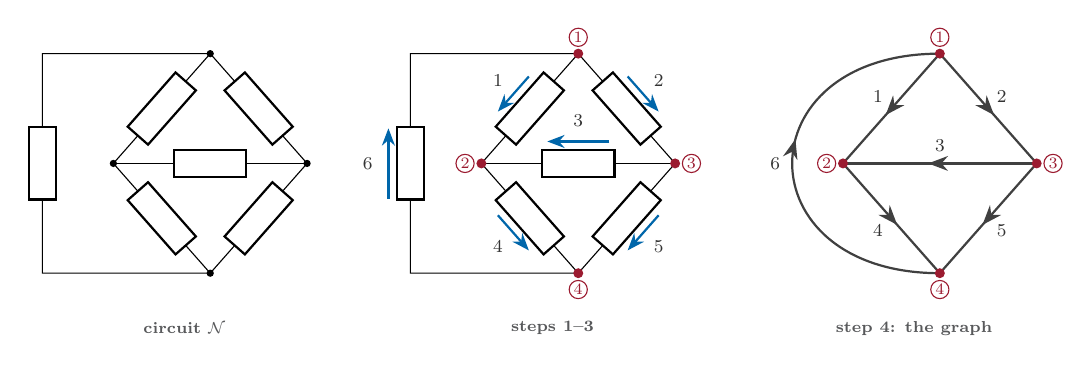
\begin{tikzpicture}[scale=0.82, transform shape]
    \begin{scope}
      \bridgecoords \bridgecircuit
      \foreach \k in {1,2,3,4} \fill (n\k) circle (1.6pt);
      \node[ttl] at (-0.4,-2.55) {circuit $\mathcal{N}$};
    \end{scope}
    \begin{scope}[xshift=5.7cm, visible on=<2->]
      \bridgecoords \bridgecircuit
      \brarr{n1}{n2}{-90}{1}  \brarr{n1}{n3}{90}{2}  \brarr{n3}{n2}{-90}{3}
      \brarr{n2}{n4}{-90}{4}  \brarr{n3}{n4}{90}{5}  \brarr{s6}{e6}{90}{6}
      \bridgenodes
      \node[ttl] at (-0.4,-2.55) {steps 1--3};
    \end{scope}
    \begin{scope}[xshift=11.3cm, visible on=<3->]
      \bridgecoords \bridgegraph
      \node[ttl] at (-0.4,-2.55) {step 4: the graph};
    \end{scope}
  \end{tikzpicture}
  \end{center}
  \vfill
  \begin{center}
    \only<1>{Six elements, drawn as boxes: their type does not matter here.}%
    \only<2>{Number the branches, give each an arrow (\Icol{current reference}), number the nodes.}%
    \only<3->{Nodes $\{\nd1,\nd2,\nd3,\nd4\}$, $n = 4$; \quad branches $\{1,\dots,6\}$, $b = 6$.\\[3pt]
      \small Branch 6 is curved only for clarity --- a straight arrow is the same graph.}
  \end{center}
  \vfill
\end{frame}

%--------------------------------------------------------------
\begin{frame}{Elements with more than two terminals}
  \vfill
  \begin{block}{A $k$-terminal element}
    Choose one terminal as its \alert{reference} (arbitrary). Draw $k-1$ branches, one
    from each other terminal to the reference terminal.
  \end{block}
  \vfill
  \begin{center}
  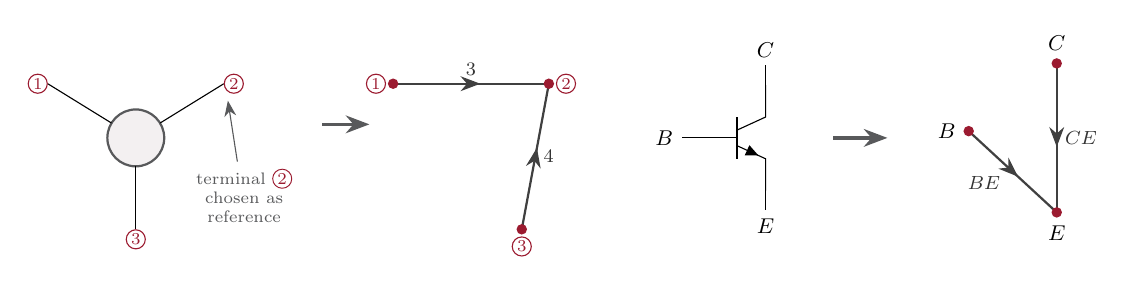
\begin{tikzpicture}[scale=0.86, transform shape]
    \begin{scope}
      \draw[elem] (0,0) circle (0.42);
      \draw (-0.36,0.22) -- (-1.3,0.8) node[nlab, left] {1};
      \draw (0.36,0.22) -- (1.3,0.8) node[nlab, right] {2};
      \draw (0,-0.42) -- (0,-1.35) node[nlab, below] {3};
      \node[capn] at (1.6,-0.85) {terminal \nd2\\ chosen as\\ reference};
      \draw[-{Stealth[length=2mm]}, metugray] (1.5,-0.35) -- (1.36,0.55);
    \end{scope}
    \draw[bigarr] (2.75,0.2) -- (3.45,0.2);
    \begin{scope}[xshift=5.1cm]
      \coordinate (t1) at (-1.3,0.8); \coordinate (t2) at (1.0,0.8); \coordinate (t3) at (0.6,-1.35);
      \draw[gbr] (t1) -- (t2);  \node[blab, above] at ($(t1)!0.5!(t2)$) {3};
      \draw[gbr] (t3) -- (t2);  \node[blab, right] at ($(t3)!0.5!(t2)$) {4};
      \foreach \k/\pos in {1/left, 2/right, 3/below}
        {\fill[metured] (t\k) circle (2.2pt); \node[nlab, \pos=3pt] at (t\k) {\k};}
    \end{scope}
    \begin{scope}[xshift=9.3cm, visible on=<3->]
      \draw (0,0) node[npn](Q){};
      \draw (Q.B) -- ++(-0.4,0) node[left, font=\small] {$B$};
      \draw (Q.C) -- ++(0,0.3) node[above, font=\small] {$C$};
      \draw (Q.E) -- ++(0,-0.3) node[below, font=\small] {$E$};
      \draw[bigarr] (1.0,0) -- (1.8,0);
      \begin{scope}[xshift=3.0cm]
        \coordinate (B) at (0,0.1); \coordinate (C) at (1.3,1.1); \coordinate (E) at (1.3,-1.1);
        \draw[gbr] (B) -- (E); \draw[gbr] (C) -- (E);
        \node[blab, below left] at ($(B)!0.45!(E)$) {$BE$};
        \node[blab, right] at ($(C)!0.5!(E)$) {$CE$};
        \foreach \p/\pos in {B/left, C/above, E/below}
          {\fill[metured] (\p) circle (2.2pt); \node[font=\small, \pos=2pt] at (\p) {$\p$};}
      \end{scope}
    \end{scope}
  \end{tikzpicture}
  \end{center}
  \vfill
  \small
  \onslide<2->
  \textbf{Why $k-1$?} KCL on a surface around the element: the $k$ terminal currents sum to
  zero, so only $k-1$ are free. By KVL, the $k-1$ voltages to the reference fix all the others.
  \onslide<3->{\ \alert{A transistor}: emitter as reference, two branches.}
  \vfill
\end{frame}

%--------------------------------------------------------------
\begin{frame}{The general case}
  \vfill
  \begin{center}
  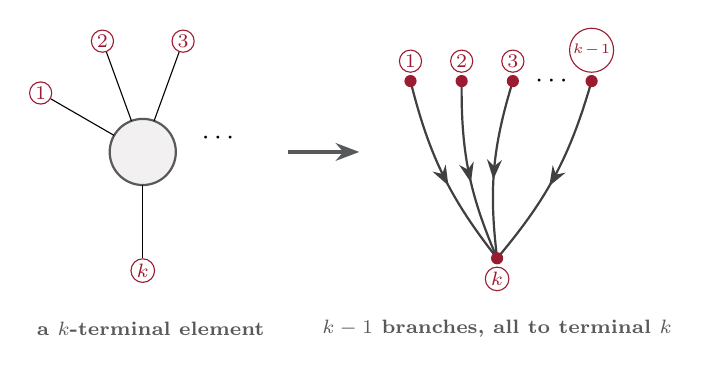
\begin{tikzpicture}[scale=1.0]
    \begin{scope}
      \draw[elem] (0,0) circle (0.42);
      \foreach \ang/\lab in {150/1, 110/2, 70/3}
        \draw (\ang:0.42) -- (\ang:1.35) node[nlab, anchor=\ang+180] {\lab};
      \draw (-90:0.42) -- (-90:1.35) node[nlab, below] {$k$};
      \node at (10:1.0) {$\cdots$};
      \node[ttl] at (0.1,-2.25) {a $k$-terminal element};
    \end{scope}
    \draw[bigarr] (1.85,0) -- (2.75,0);
    \begin{scope}[xshift=4.5cm]
      \coordinate (k) at (0,-1.35);
      \foreach \x/\lab in {-1.1/1, -0.45/2, 0.2/3}
        {\coordinate (u) at (\x,0.9);
         \draw[gbr] (u) to[bend right=12] (k);
         \fill[metured] (u) circle (2.2pt); \node[nlab, above=3pt] at (u) {\lab};}
      \coordinate (u) at (1.2,0.9);
      \draw[gbr] (u) to[bend left=12] (k);
      \fill[metured] (u) circle (2.2pt); \node[nlab, above=3pt, font=\tiny] at (u) {$k\!-\!1$};
      \node at (0.72,0.9) {$\cdots$};
      \fill[metured] (k) circle (2.2pt); \node[nlab, below=3pt] at (k) {$k$};
      \node[ttl] at (0,-2.25) {$k-1$ branches, all to terminal $k$};
    \end{scope}
  \end{tikzpicture}
  \end{center}
  \vfill
  \begin{center}\small
    A dependent source needs nothing new: it is already two branches ---\\
    the branch that senses the controlling variable, and the source branch.
  \end{center}
  \vfill
\end{frame}

%--------------------------------------------------------------
\begin{frame}{Example: a circuit with a 3-terminal element}
  \vfill
  \begin{center}
  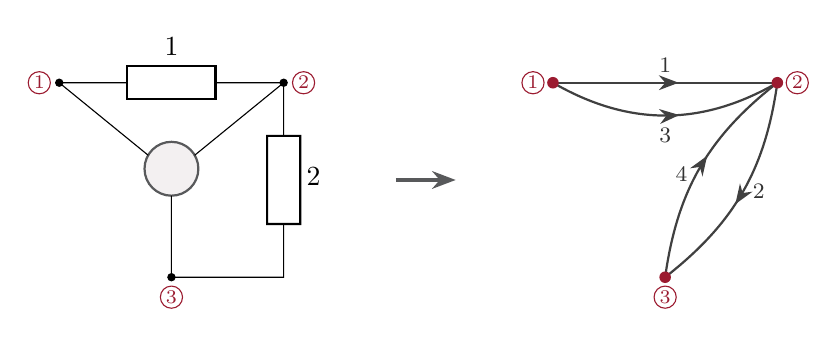
\begin{tikzpicture}[scale=0.95]
    \begin{scope}
      \coordinate (a) at (0,1.6); \coordinate (b) at (3,1.6); \coordinate (c) at (1.5,-1.0);
      \draw (a) to[generic, l=1] (b);
      \draw (b) to[generic, l=2] (3,-1.0) -- (c);
      \draw[elem] (1.5,0.45) circle (0.36);
      \draw (a) -- (1.19,0.63); \draw (b) -- (1.81,0.63); \draw (1.5,0.09) -- (c);
      \foreach \p/\k/\pos in {a/1/left, b/2/right, c/3/below}
        {\fill (\p) circle (1.6pt); \node[nlab, \pos=3pt] at (\p) {\k};}
    \end{scope}
    \draw[bigarr, visible on=<2->] (4.5,0.3) -- (5.3,0.3);
    \begin{scope}[xshift=6.6cm, visible on=<2->]
      \coordinate (a) at (0,1.6); \coordinate (b) at (3,1.6); \coordinate (c) at (1.5,-1.0);
      \draw[gbr] (a) -- (b);                \node[blab, above] at (1.5,1.6) {1};
      \draw[gbr] (c) to[bend left=22] (b);  \node[blab] at (1.72,0.38) {4};
      \draw[gbr] (a) to[bend right=30] (b); \node[blab] at (1.5,0.9) {3};
      \draw[gbr] (b) to[bend left=22] (c);  \node[blab] at (2.75,0.15) {2};
      \foreach \p/\k/\pos in {a/1/left, b/2/right, c/3/below}
        {\fill[metured] (\p) circle (2.2pt); \node[nlab, \pos=3pt] at (\p) {\k};}
    \end{scope}
  \end{tikzpicture}
  \end{center}
  \vfill
  \begin{center}\small
    \only<1>{Elements 1 and 2 have two terminals; the circle has three. Find the graph.}%
    \only<2->{Elements 1, 2: one branch each. 3-terminal element, reference terminal at \nd2:
      branches 3 (\nd1$\to$\nd2) and 4 (\nd3$\to$\nd2).\\[3pt]
      $n = 3$, $b = 4$. Two branches may join the same pair of nodes.}
  \end{center}
  \vfill
\end{frame}

%--------------------------------------------------------------
\begin{frame}{KCL on a circuit graph}
  \vfill
  \begin{columns}[c,onlytextwidth]
    \begin{column}{0.42\textwidth}
      \begin{center}
      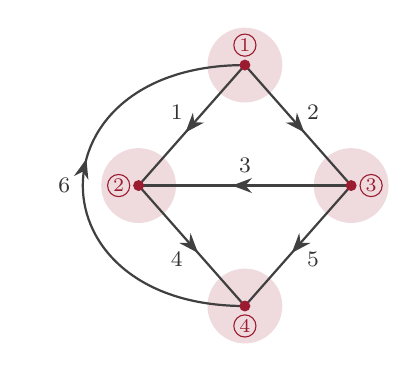
\begin{tikzpicture}[scale=0.9]
        \bridgecoords
        \node[halo, visible on=<2>] at (n1) {};
        \node[halo, visible on=<3>] at (n2) {};
        \node[halo, visible on=<4>] at (n3) {};
        \node[halo, visible on=<5>] at (n4) {};
        \bridgegraph
      \end{tikzpicture}
      \end{center}
    \end{column}
    \begin{column}{0.56\textwidth}
      \small
      Current along its arrow. At each node:\\
      \alert{leaving $+$}, \ \alert{entering $-$}, \ sum $= 0$.
      \[
      \renewcommand{\arraystretch}{1.35}
      \begin{array}{c@{\;\;}r@{\;}r@{\;}r@{\;}r@{\;}r@{\;}r@{\;}l}
        \U2{\nd1:} & \U2{\Icol{i_1}} & \U2{+\Icol{i_2}} & & & & \U2{-\Icol{i_6}} & \U2{=0}\\
        \U3{\nd2:} & \U3{-\Icol{i_1}} & & \U3{-\Icol{i_3}} & \U3{+\Icol{i_4}} & & & \U3{=0}\\
        \U4{\nd3:} & & \U4{-\Icol{i_2}} & \U4{+\Icol{i_3}} & & \U4{+\Icol{i_5}} & & \U4{=0}\\
        \U5{\nd4:} & & & & \U5{-\Icol{i_4}} & \U5{-\Icol{i_5}} & \U5{+\Icol{i_6}} & \U5{=0}
      \end{array}
      \]
      \onslide<6->
      Only the \alert{graph} was used. Same graph $\Rightarrow$ same KCL equations,
      whatever the elements are.
    \end{column}
  \end{columns}
  \vfill
\end{frame}

%--------------------------------------------------------------
\begin{frame}{From equations to a matrix}
  \vfill
  \begin{center}
  \small
  Only $+1$, $-1$ and $0$ appear. Rows: nodes. Columns: branches.
  \end{center}
  \vfill
  \[
    \incmat{Aa}{6}{1,2,3,4}{%
       1 \&  1 \&  0 \&  0 \&  0 \& -1\\
      -1 \&  0 \& -1 \&  1 \&  0 \&  0\\
       0 \& -1 \&  1 \&  0 \&  1 \&  0\\
       0 \&  0 \&  0 \& -1 \& -1 \&  1\\}{%
      \only<2>{\draw[metured, thick, rounded corners=2pt]
        ([xshift=-2pt,yshift=1pt]Aa-1-1.north west) rectangle ([xshift=2pt,yshift=-1pt]Aa-1-6.south east);}
      \only<3>{\draw[metured, thick, rounded corners=2pt]
        ([xshift=-2pt,yshift=1pt]Aa-1-3.north west) rectangle ([xshift=2pt,yshift=-1pt]Aa-4-3.south east);}}
    \;
    \begin{bmatrix}
      \Icol{i_1}\\ \Icol{i_2}\\ \Icol{i_3}\\ \Icol{i_4}\\ \Icol{i_5}\\ \Icol{i_6}
    \end{bmatrix}
    =
    \begin{bmatrix} 0\\ 0\\ 0\\ 0 \end{bmatrix}
    \qquad\Longleftrightarrow\qquad
    \alert{A_a\,\Icol{\mathbf{i}} = \mathbf{0}}
  \]
  \vfill
  \begin{center}\small
    \only<1>{A matrix that stores the graph: a \alert{circuit matrix}. This one is the first and most basic.}%
    \only<2>{\alert{A row is a node}: row \nd1 times $\Icol{\mathbf{i}}$ is KCL at \nd1.}%
    \only<3->{\alert{A column is a branch}: one $+1$ (leaves) and one $-1$ (enters).
      Column 3: from \nd3 to \nd2.}
  \end{center}
  \vfill
\end{frame}

%--------------------------------------------------------------
\begin{frame}{The incidence matrix}
  \vfill
  \begin{block}{Incidence matrix $A_a$ \ ($n \times b$)}
    \[
      a_{ij} =
      \begin{cases}
        +1 & \text{if branch } j \text{ leaves node } i,\\
        -1 & \text{if branch } j \text{ enters node } i,\\
        \phantom{+}0 & \text{otherwise.}
      \end{cases}
    \]
    With $\Icol{\mathbf{i}} = [\,\Icol{i_1}\ \cdots\ \Icol{i_b}\,]^{T}$, the
    \alert{branch current vector}: KCL at every node is $A_a\Icol{\mathbf{i}} = \mathbf{0}$.
  \end{block}
  \vfill
  \small
  \begin{itemize}\itemsep4pt
    \item The subscript $a$: \emph{all} nodes have a row.
    \item<2-> The columns hold the whole graph: from $A_a$ alone you can redraw it, arrows included.
    \item<3-> Reversing an arrow flips the sign of that column --- nothing else changes.
  \end{itemize}
  \vfill
\end{frame}

%--------------------------------------------------------------
\begin{frame}{Review: linear dependence}
  \vfill
  \begin{block}{Linear dependence}
    $\mathbf{v}_1, \dots, \mathbf{v}_k$ (same size) are \alert{linearly dependent} if there
    are real $\alpha_1, \dots, \alpha_k$, \textbf{not all zero}, with
    $\alpha_1\mathbf{v}_1 + \dots + \alpha_k\mathbf{v}_k = \mathbf{0}$. Otherwise they are
    \alert{linearly independent}.
  \end{block}
  \vfill
  \begin{columns}[t,onlytextwidth]
    \begin{column}{0.38\textwidth}
      \onslide<2->
      \[ \begin{bmatrix} 1\\ 0 \end{bmatrix},\ \begin{bmatrix} 0\\ -1 \end{bmatrix} \]
      \small independent: $[\alpha_1\ \ {-\alpha_2}]^T = \mathbf{0}$ only if both are zero.
    \end{column}
    \begin{column}{0.58\textwidth}
      \onslide<3->
      \[ \mathbf{v}_1 = \begin{bmatrix} 1\\ 2\\ 3 \end{bmatrix},\
         \mathbf{v}_2 = \begin{bmatrix} 4\\ 5\\ 6 \end{bmatrix},\
         \mathbf{v}_3 = \begin{bmatrix} 7\\ 8\\ 9 \end{bmatrix} \]
      \small dependent: $\mathbf{v}_1 - 2\mathbf{v}_2 + \mathbf{v}_3 = \mathbf{0}$, so
      $\mathbf{v}_3 = 2\mathbf{v}_2 - \mathbf{v}_1$.
    \end{column}
  \end{columns}
  \vfill
  \onslide<4->
  \begin{center}\small
    Rows of $M$ dependent $\Rightarrow$ one equation of $M\mathbf{x} = \mathbf{0}$ follows from the
    others.\\ Number of independent rows: the \alert{rank}. All rows independent: \alert{full row rank}.
  \end{center}
  \vfill
\end{frame}

%--------------------------------------------------------------
\begin{frame}{The rows of $A_a$ are always dependent}
  \vfill
  \begin{center}
    Every column has one $+1$ and one $-1$, so
    \[ \text{row } \nd1 + \text{row } \nd2 + \dots + \text{row } \nd{$n$} = [\,0\ 0\ \cdots\ 0\,] \]
    --- dependence with every $\alpha = 1$. One KCL equation is always redundant.
  \end{center}
  \vfill
  \onslide<2->
  \begin{block}{Reduced incidence matrix $A$ \ ($(n-1) \times b$)}
    Choose a \alert{reference node} (\alert{ground}), arbitrarily. Delete its row from $A_a$.
  \end{block}
  \vfill
  \begin{center}\small
    The reference node is also the common reference for node voltages.
  \end{center}
  \vfill
\end{frame}

%--------------------------------------------------------------
\begin{frame}{Example: the reduced incidence matrix of $\mathcal{N}$}
  \vfill
  \begin{columns}[c,onlytextwidth]
    \begin{column}{0.3\textwidth}
      \begin{center}
      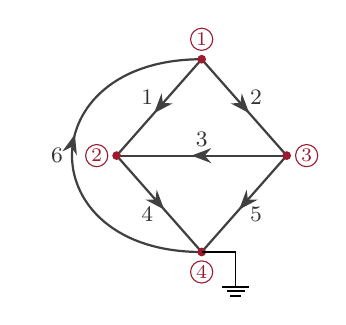
\begin{tikzpicture}[scale=0.72]
        \bridgecoords
        \bridgegraph
        \draw (n4) -- ++(0.6,0) -- ++(0,-0.15) node[ground, scale=0.8]{};
      \end{tikzpicture}
      \end{center}
    \end{column}
    \begin{column}{0.68\textwidth}
      \small
      Reference node: \nd4.
      \[
        A_a =
        \begin{bmatrix}
           1 &  1 &  0 &  0 &  0 & -1\\
          -1 &  0 & -1 &  1 &  0 &  0\\
           0 & -1 &  1 &  0 &  1 &  0\\
           \rowcolor{metured!14}
           0 &  0 &  0 & -1 & -1 &  1
        \end{bmatrix}
      \]
      \onslide<2->
      \[
        A =
        \begin{bmatrix}
           1 &  1 &  0 &  0 &  0 & -1\\
          -1 &  0 & -1 &  1 &  0 &  0\\
           0 & -1 &  1 &  0 &  1 &  0
        \end{bmatrix}
        \qquad (3 \times 6)
      \]
      \onslide<3->
      Rows independent: columns 6, 4, 5 each have a single nonzero entry, in rows
      \nd1, \nd2, \nd3.
    \end{column}
  \end{columns}
  \vfill
\end{frame}

%--------------------------------------------------------------
\begin{frame}{Deleting the row loses nothing}
  \vfill
  \begin{block}{No equation is lost}
    $A\Icol{\mathbf{i}} = \mathbf{0} \;\Rightarrow\; A_a\Icol{\mathbf{i}} = \mathbf{0}$:
    the deleted row is minus the sum of the rows that were kept.
  \end{block}
  \vfill
  \onslide<2->
  \begin{block}{No part of the graph is lost}
    Each column of $A_a$ sums to zero, so the deleted row can be rebuilt from $A$.\\
    A column of $A$ with a single nonzero entry is a branch that touches the reference node.
  \end{block}
  \vfill
\end{frame}

%--------------------------------------------------------------
\begin{frame}{Connected graphs}
  \vfill
  \begin{block}{Connected graph}
    Any two nodes are joined by a path of branches, ignoring the arrow directions.
  \end{block}
  \vfill
  \begin{center}
  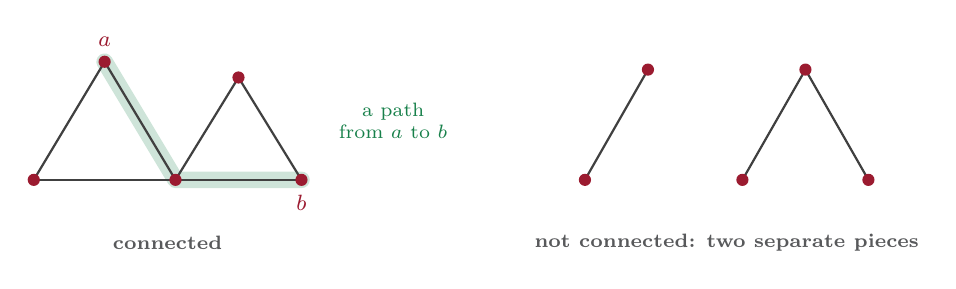
\begin{tikzpicture}[scale=1.0]
    \begin{scope}
      \coordinate (a) at (0.9,1.5); \coordinate (p) at (0,0); \coordinate (q) at (1.8,0);
      \coordinate (b) at (3.4,0);   \coordinate (r) at (2.6,1.3);
      \draw[hal, visible on=<2->] (a) -- (q) -- (b);
      \foreach \u/\v in {a/p, a/q, p/q, q/b, q/r, r/b}
        \draw[black!75, thick] (\u) -- (\v);
      \foreach \p in {a,p,q,b,r} \fill[metured] (\p) circle (2.2pt);
      \node[glab, above=2pt] at (a) {$a$}; \node[glab, below=2pt] at (b) {$b$};
      \node[capn, text=cpow, anchor=west, visible on=<2->] at (3.75,0.75) {a path\\ from $a$ to $b$};
      \node[ttl] at (1.7,-0.8) {connected};
    \end{scope}
    \begin{scope}[xshift=7.0cm]
      \coordinate (p) at (0,0); \coordinate (q) at (0.8,1.4);
      \coordinate (r) at (2.0,0); \coordinate (s) at (2.8,1.4); \coordinate (t) at (3.6,0);
      \draw[black!75, thick] (p) -- (q);
      \draw[black!75, thick] (r) -- (s) -- (t);
      \foreach \p in {p,q,r,s,t} \fill[metured] (\p) circle (2.2pt);
      \node[ttl] at (1.8,-0.8) {not connected: two separate pieces};
    \end{scope}
  \end{tikzpicture}
  \end{center}
  \vfill
\end{frame}

%--------------------------------------------------------------
\begin{frame}{Connected graph $\Rightarrow$ rows of $A$ independent}
  \vfill
  \begin{block}{Full row rank}
    If the graph is connected, the $n-1$ rows of $A$ are linearly independent:
    $\operatorname{rank} A = n - 1$.
  \end{block}
  \vfill
  \small
  \onslide<2->
  \textbf{Why.} Suppose $\sum \alpha\,(\text{rows of } A) = 0$; the reference node has no row,
  give it $\alpha = 0$.
  \begin{itemize}
    \item A branch from $p$ to $q$ gives $\alpha_p - \alpha_q = 0$: neighbours have equal $\alpha$.
    \item Connected: every node has a path to the reference, so every $\alpha = 0$.
  \end{itemize}
  \vfill
  \onslide<3->
  \textbf{Two separate pieces} (for example, coupled only through a transformer): the other
  piece keeps its own dependence. Join the pieces with \alert{one wire} --- by KCL it carries
  no current, so nothing changes. In EE201 all graphs are connected.
  \vfill
\end{frame}

%--------------------------------------------------------------
\begin{frame}{KCL of a circuit graph}
  \vfill
  \begin{center}
  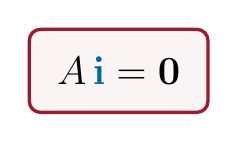
\begin{tikzpicture}
    \node[draw=metured, very thick, rounded corners=4pt, fill=metured!5, inner sep=10pt] {%
      \Large $A\,\Icol{\mathbf{i}} = \mathbf{0}$};
  \end{tikzpicture}
  \end{center}
  \vfill
  \begin{center}
  \begin{tabular}{@{}l l@{}}
    $A \in \mathbb{R}^{(n-1)\times b}$ & reduced incidence matrix\\[3pt]
    $\Icol{\mathbf{i}} \in \mathbb{R}^{b}$ & branch current vector
  \end{tabular}
  \end{center}
  \vfill
  \begin{center}
    For a connected graph: $n-1$ \alert{independent} KCL equations,\\
    and every other KCL equation of the circuit follows from them.
  \end{center}
  \vfill
\end{frame}

%--------------------------------------------------------------
\begin{frame}{Example: KCL for the circuit with a 3-terminal element}
  \vfill
  \begin{columns}[c,onlytextwidth]
    \begin{column}{0.36\textwidth}
      \begin{center}
      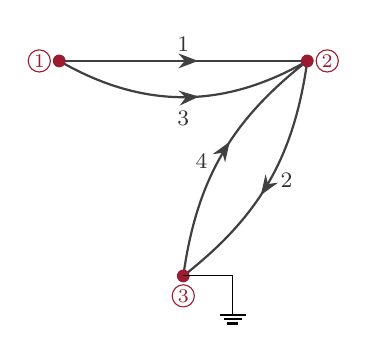
\begin{tikzpicture}[scale=1.05]
        \coordinate (a) at (0,1.6); \coordinate (b) at (3,1.6); \coordinate (c) at (1.5,-1.0);
        \draw[gbr] (a) -- (b);                \node[blab, above] at (1.5,1.6) {1};
        \draw[gbr] (c) to[bend left=22] (b);  \node[blab] at (1.72,0.38) {4};
        \draw[gbr] (a) to[bend right=30] (b); \node[blab] at (1.5,0.9) {3};
        \draw[gbr] (b) to[bend left=22] (c);  \node[blab] at (2.75,0.15) {2};
        \foreach \p/\k/\pos in {a/1/left, b/2/right, c/3/below}
          {\fill[metured] (\p) circle (2.2pt); \node[nlab, \pos=3pt] at (\p) {\k};}
        \draw (c) -- ++(0.6,0) -- ++(0,-0.15) node[ground, scale=0.8]{};
      \end{tikzpicture}
      \end{center}
      \begin{center}\small Reference node: \nd3.\end{center}
    \end{column}
    \begin{column}{0.62\textwidth}
      \onslide<2->
      \[
        A_a =
        \incmat{Ab}{4}{1,2,3}{%
           1 \&  0 \&  1 \&  0\\
          -1 \&  1 \& -1 \& -1\\
           0 \& -1 \&  0 \&  1\\}{}
      \]
      \onslide<3->
      \[
        A =
        \begin{bmatrix}
           1 &  0 &  1 &  0\\
          -1 &  1 & -1 & -1
        \end{bmatrix}
      \]
      \onslide<4->
      \small
      \[ \Icol{i_1} + \Icol{i_3} = 0, \qquad -\Icol{i_1} + \Icol{i_2} - \Icol{i_3} - \Icol{i_4} = 0 \]
      Columns 1 and 3 are equal: same nodes, same direction.\\
      Reference terminal (\nd2) and reference node (\nd3): two separate choices.
    \end{column}
  \end{columns}
  \vfill
\end{frame}

%--------------------------------------------------------------
\begin{frame}{Summary}
  \vfill
  \begin{itemize}\itemsep5pt
    \item $2b$ equations: $b$ \textbf{element} equations and $b$ \textbf{interconnection}
          equations (KCL, KVL). The second group depends only on the \alert{graph}.
    \item The graph: number the branches, give each an arbitrary arrow, number the nodes.
          A $k$-terminal element becomes $k-1$ branches.
    \item \textbf{Incidence matrix} $A_a$ ($n \times b$): $+1$ leaves, $-1$ enters.
          KCL: $A_a\Icol{\mathbf{i}} = \mathbf{0}$. Its rows always sum to zero.
    \item \textbf{Reduced incidence matrix} $A$: delete the reference node's row. For a
          \alert{connected} graph, $A\Icol{\mathbf{i}} = \mathbf{0}$ gives exactly the $n-1$
          independent KCL equations.
  \end{itemize}
  \vfill
\end{frame}

%--------------------------------------------------------------
\begin{frame}{Next lecture}
  \vfill
  \begin{center}
  \begin{block}{KVL on the graph}
    Every branch voltage is a difference of \alert{node voltages}:
    $\Vcol{\mathbf{v}} = A^{T}\mathbf{e}$ --- the same matrix $A$, transposed.
    Then Tellegen's theorem, in one line from $A\Icol{\mathbf{i}} = \mathbf{0}$ and $\Vcol{\mathbf{v}} = A^{T}\mathbf{e}$.
  \end{block}
  \end{center}
  \vfill
  \begin{center}
    {\Large\color{metured} Questions?}
  \end{center}
  \vfill
\end{frame}

\end{document}
